\documentclass[10pt]{article}
\usepackage[margin=18mm]{geometry}
\usepackage{graphicx,booktabs,hyperref}
\usepackage[strings]{underscore}
\setlength{\parindent}{0pt}\setlength{\parskip}{5pt}
\begin{document}
\section*{Retained complete-DLP setup refusals}

The frozen structured K0 n=17 request is refused by the registered curve
constructor: it has no usable prime subgroup under this constructor.
No session or measured cost was produced. It does not stand for a zero-cost
result or an excluded field in the mathematics.

\begin{center}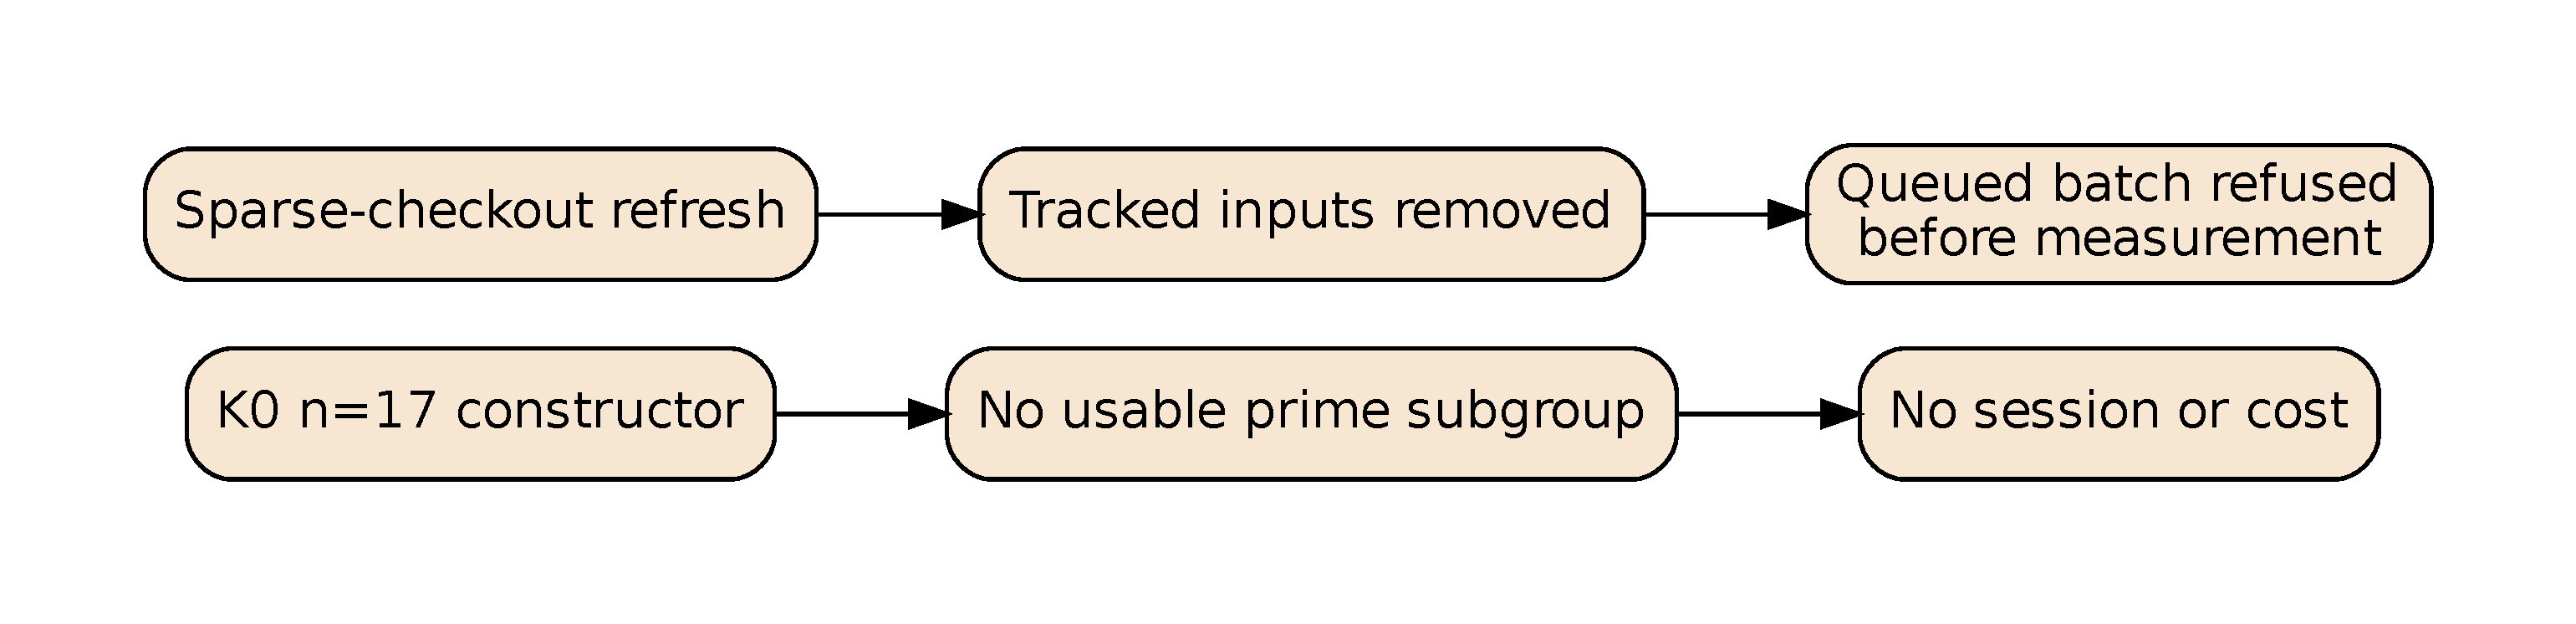
\includegraphics[width=.98\linewidth]{refusals.pdf}\end{center}

After the n=23 replay completed, a metadata-oriented sparse-checkout refresh
had removed previously force-added tracked study inputs. The queued first
quartic smoke and three HKY setup commands consequently refused before
native measurement. Their console logs and partial launch metadata remain
in pipeline-receipts/setup-sparse-refusal-20261025 and the failed -01
directories. All required study paths were restored, and a fresh -02 batch
was launched with explicit file preflight. The active frozen runner was
not edited. The successful restart is a separate run, never a replacement
of these refusals. No scientific verdict follows from absent input files.

Raw constructor error: evidence/checks/ic-pipeline-n17-20261025.log.
Original commands and runner snapshots are in evidence/runners and the
launch receipts. Full source revisions, hashes and native stdout/stderr
are retained for actual measurements. These are setup outcomes, with no
comparable numerical samples, so the visual is a process diagram.

\end{document}
